\documentclass{standalone}
\usepackage{tikz}
\usetikzlibrary{patterns, positioning}
\usepackage[sfdefault]{ClearSans} %% option 'sfdefault' activates Clear Sans as the default text font
\usepackage[T1]{fontenc}

\begin{document}
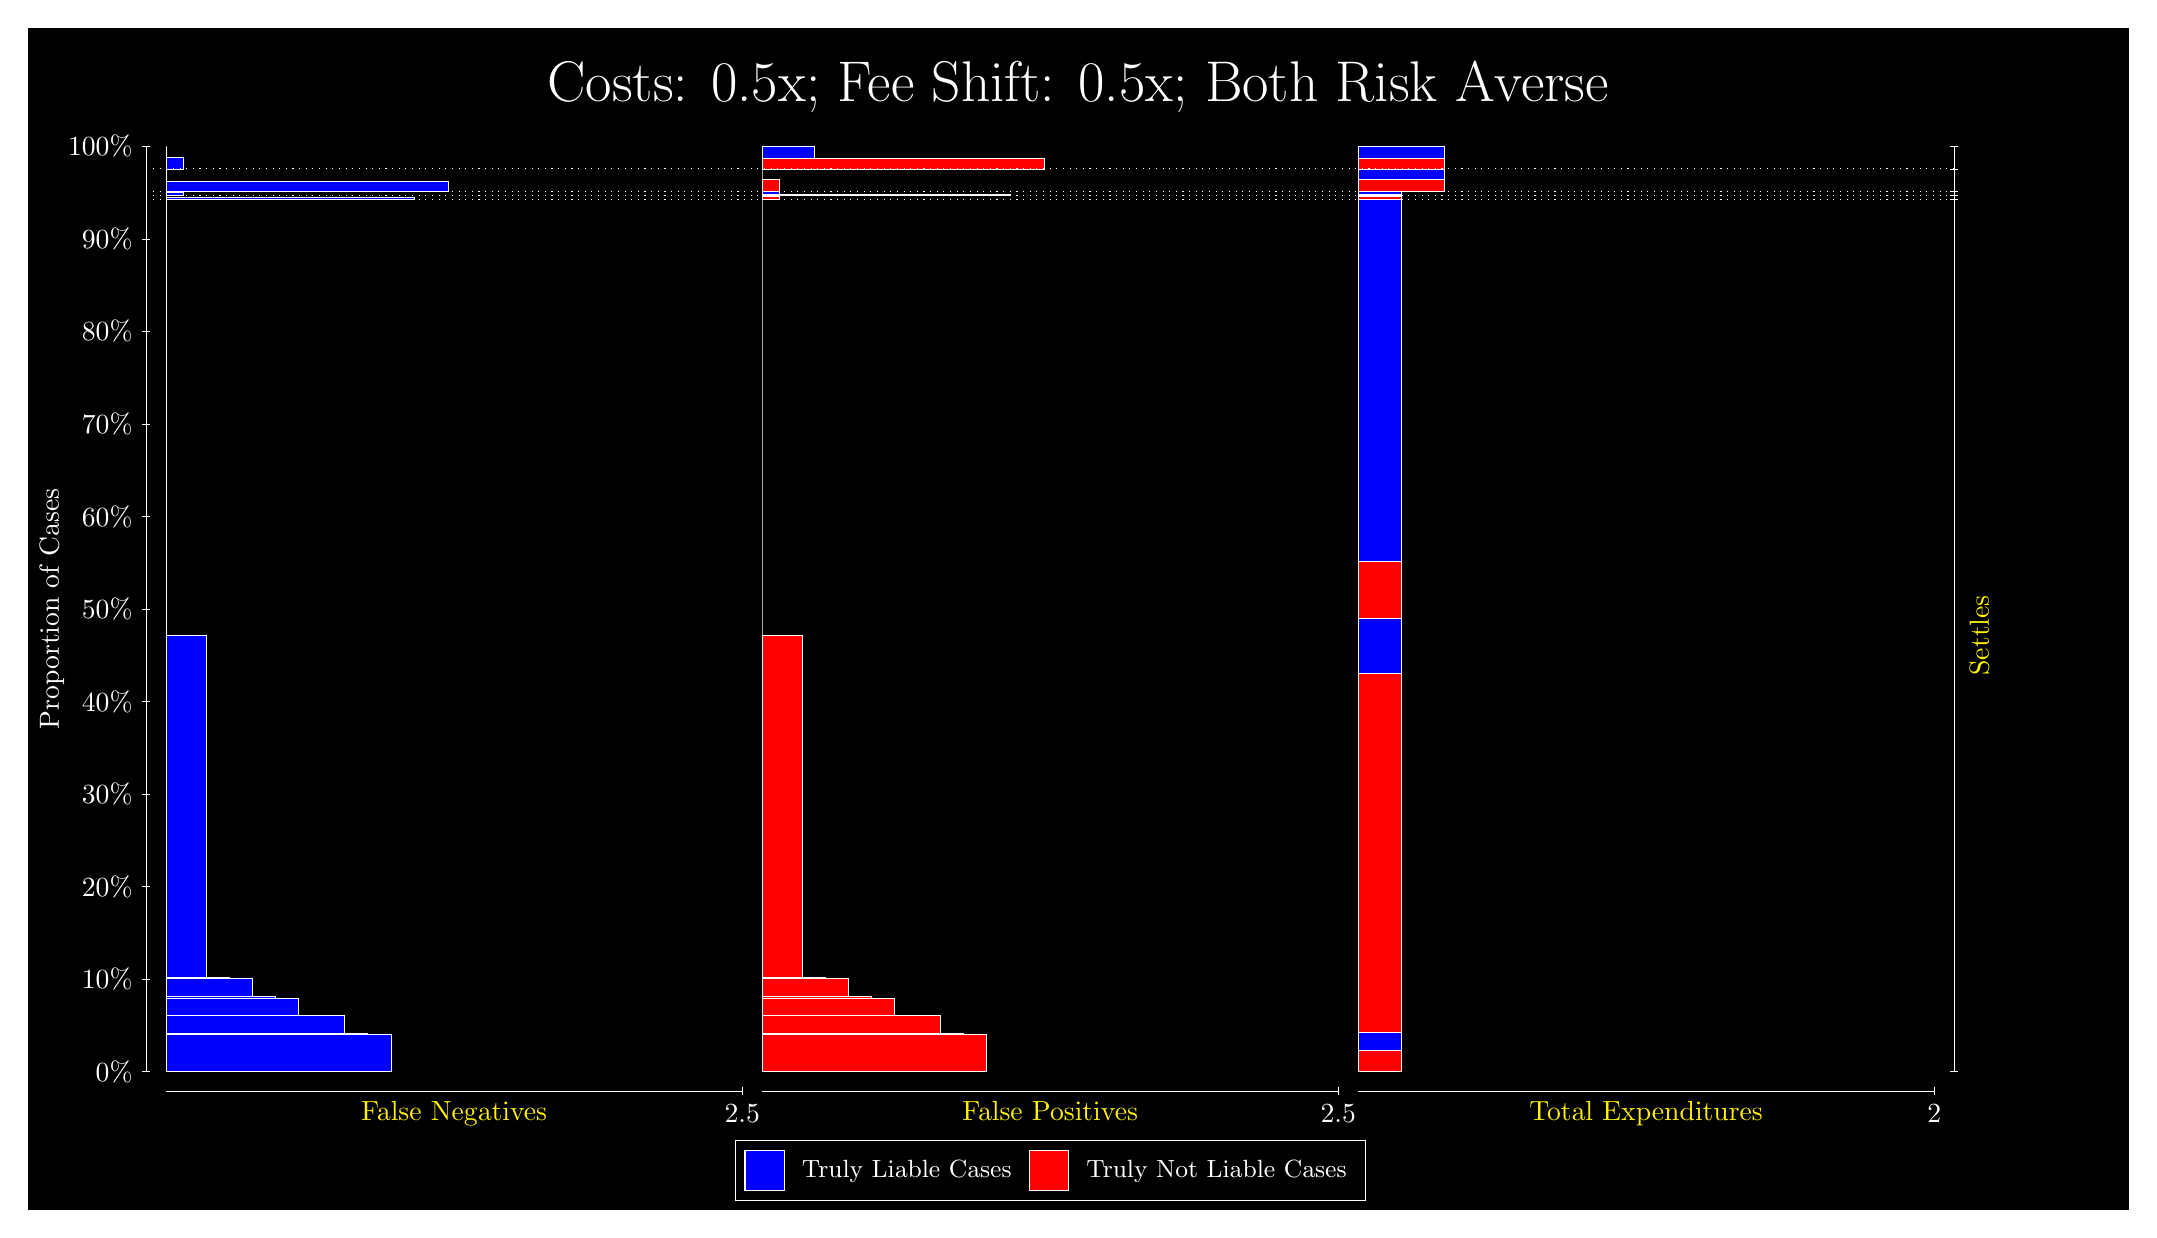
\begin{tikzpicture}
\draw[fill=black] (0,0) rectangle (26.667,15);
\draw[text=white] (0,13.5) rectangle (26.667,15) node[midway] {\huge Costs: 0.5x; Fee Shift: 0.5x; Both Risk Averse};
\draw[white, very thin] (1.5,1.75) -- (1.5,13.5);
\node[rotate=90, text=white, anchor=center] at (0.3, 7.625) {Proportion of Cases};
\draw[white, very thin] (1.45,1.75) -- (1.55,1.75);
\node[text=white, anchor=east] at (1.45, 1.75) {0\%};
\draw[white, very thin] (1.45,2.925) -- (1.55,2.925);
\node[text=white, anchor=east] at (1.45, 2.925) {10\%};
\draw[white, very thin] (1.45,4.1) -- (1.55,4.1);
\node[text=white, anchor=east] at (1.45, 4.1) {20\%};
\draw[white, very thin] (1.45,5.275) -- (1.55,5.275);
\node[text=white, anchor=east] at (1.45, 5.275) {30\%};
\draw[white, very thin] (1.45,6.45) -- (1.55,6.45);
\node[text=white, anchor=east] at (1.45, 6.45) {40\%};
\draw[white, very thin] (1.45,7.625) -- (1.55,7.625);
\node[text=white, anchor=east] at (1.45, 7.625) {50\%};
\draw[white, very thin] (1.45,8.8) -- (1.55,8.8);
\node[text=white, anchor=east] at (1.45, 8.8) {60\%};
\draw[white, very thin] (1.45,9.975) -- (1.55,9.975);
\node[text=white, anchor=east] at (1.45, 9.975) {70\%};
\draw[white, very thin] (1.45,11.15) -- (1.55,11.15);
\node[text=white, anchor=east] at (1.45, 11.15) {80\%};
\draw[white, very thin] (1.45,12.325) -- (1.55,12.325);
\node[text=white, anchor=east] at (1.45, 12.325) {90\%};
\draw[white, very thin] (1.45,13.5) -- (1.55,13.5);
\node[text=white, anchor=east] at (1.45, 13.5) {100\%};

\draw[white, very thin] (24.457,1.75) -- (24.457,13.5);
\draw[white, very thin] (24.407,1.75) -- (24.507,1.75);
\node[anchor=west] at (24.407, 1.75) {};
\draw[white, very thin] (24.407,12.829) -- (24.507,12.829);
\node[anchor=west] at (24.407, 12.829) {};
\draw[white, very thin] (24.407,12.879) -- (24.507,12.879);
\node[anchor=west] at (24.407, 12.879) {};
\draw[white, very thin] (24.407,12.929) -- (24.507,12.929);
\node[anchor=west] at (24.407, 12.929) {};
\draw[white, very thin] (24.407,13.214) -- (24.507,13.214);
\node[anchor=west] at (24.407, 13.214) {};
\draw[white, very thin] (24.407,13.5) -- (24.507,13.5);
\node[anchor=west] at (24.407, 13.5) {};

\draw[white, very thin, fill=blue] (1.75,1.75) rectangle (4.6044,2.2262);
\draw[white, very thin, fill=blue] (1.75,2.2262) rectangle (4.3116,2.2336);
\draw[white, very thin, fill=blue] (1.75,2.2336) rectangle (4.0188,2.459);
\draw[white, very thin, fill=blue] (1.75,2.459) rectangle (3.7261,2.4663);
\draw[white, very thin, fill=blue] (1.75,2.4663) rectangle (3.4333,2.6848);
\draw[white, very thin, fill=blue] (1.75,2.6848) rectangle (3.1406,2.7003);
\draw[white, very thin, fill=blue] (1.75,2.7003) rectangle (2.8478,2.9338);
\draw[white, very thin, fill=blue] (1.75,2.9338) rectangle (2.5551,2.9492);
\draw[white, very thin, fill=blue] (1.75,2.9492) rectangle (2.2623,7.2894);
\draw[white, very thin, fill=red] (1.75,7.2894) rectangle (1.75,12.829);
\draw[white, very thin, fill=blue] (1.75,12.829) rectangle (4.8971,12.847);
\draw[white, very thin, fill=red] (1.75,12.847) rectangle (1.75,12.879);
\draw[white, very thin, fill=blue] (1.75,12.879) rectangle (1.9696,12.911);
\draw[white, very thin, fill=red] (1.75,12.911) rectangle (1.75,12.929);
\draw[white, very thin, fill=blue] (1.75,12.929) rectangle (5.3362,13.062);
\draw[white, very thin, fill=red] (1.75,13.062) rectangle (1.75,13.214);
\draw[white, very thin, fill=blue] (1.75,13.214) rectangle (1.9696,13.367);
\draw[white, very thin, fill=red] (1.75,13.367) rectangle (1.75,13.5);
\draw[white, very thin, fill=red] (9.3189,1.75) rectangle (12.173,2.2262);
\draw[white, very thin, fill=red] (9.3189,2.2262) rectangle (11.88,2.2336);
\draw[white, very thin, fill=red] (9.3189,2.2336) rectangle (11.588,2.459);
\draw[white, very thin, fill=red] (9.3189,2.459) rectangle (11.295,2.4663);
\draw[white, very thin, fill=red] (9.3189,2.4663) rectangle (11.002,2.6848);
\draw[white, very thin, fill=red] (9.3189,2.6848) rectangle (10.709,2.7003);
\draw[white, very thin, fill=red] (9.3189,2.7003) rectangle (10.417,2.9338);
\draw[white, very thin, fill=red] (9.3189,2.9338) rectangle (10.124,2.9492);
\draw[white, very thin, fill=red] (9.3189,2.9492) rectangle (9.8312,7.2894);
\draw[white, very thin, fill=blue] (9.3189,7.2894) rectangle (9.3189,12.829);
\draw[white, very thin, fill=red] (9.3189,12.829) rectangle (9.5384,12.861);
\draw[white, very thin, fill=blue] (9.3189,12.861) rectangle (9.3189,12.879);
\draw[white, very thin, fill=red] (9.3189,12.879) rectangle (12.466,12.897);
\draw[white, very thin, fill=blue] (9.3189,12.897) rectangle (9.5384,12.929);
\draw[white, very thin, fill=red] (9.3189,12.929) rectangle (9.5384,13.081);
\draw[white, very thin, fill=blue] (9.3189,13.081) rectangle (9.3189,13.214);
\draw[white, very thin, fill=red] (9.3189,13.214) rectangle (12.905,13.348);
\draw[white, very thin, fill=blue] (9.3189,13.348) rectangle (9.9776,13.5);
\draw[white, very thin, fill=red] (16.888,1.75) rectangle (17.437,2.0144);
\draw[white, very thin, fill=blue] (16.888,2.0144) rectangle (17.437,2.2544);
\draw[white, very thin, fill=red] (16.888,2.2544) rectangle (17.437,6.8132);
\draw[white, very thin, fill=blue] (16.888,6.8132) rectangle (17.437,7.508);
\draw[white, very thin, fill=red] (16.888,7.508) rectangle (17.437,8.2243);
\draw[white, very thin, fill=blue] (16.888,8.2243) rectangle (17.437,12.829);
\draw[white, very thin, fill=red] (16.888,12.829) rectangle (17.437,12.861);
\draw[white, very thin, fill=blue] (16.888,12.861) rectangle (17.437,12.879);
\draw[white, very thin, fill=red] (16.888,12.879) rectangle (17.437,12.897);
\draw[white, very thin, fill=blue] (16.888,12.897) rectangle (17.437,12.929);
\draw[white, very thin, fill=red] (16.888,12.929) rectangle (17.986,13.081);
\draw[white, very thin, fill=blue] (16.888,13.081) rectangle (17.986,13.214);
\draw[white, very thin, fill=red] (16.888,13.214) rectangle (17.986,13.348);
\draw[white, very thin, fill=blue] (16.888,13.348) rectangle (17.986,13.5);
\draw[white, dotted] (1.5,12.829) -- (24.457,12.829);
\draw[white, dotted] (1.5,12.879) -- (24.457,12.879);
\draw[white, dotted] (1.5,12.929) -- (24.457,12.929);
\draw[white, dotted] (1.5,13.214) -- (24.457,13.214);
\draw[white, very thin] (1.75,1.5) -- (9.0689,1.5);
\node[text=yellow, anchor=north] at (5.4094, 1.5) {False Negatives};
\draw[white, very thin] (9.0689,1.45) -- (9.0689,1.55);
\node[text=white, anchor=north] at (9.0689, 1.45) {2.5};

\draw[white, very thin] (9.3189,1.5) -- (16.638,1.5);
\node[text=yellow, anchor=north] at (12.978, 1.5) {False Positives};
\draw[white, very thin] (16.638,1.45) -- (16.638,1.55);
\node[text=white, anchor=north] at (16.638, 1.45) {2.5};

\draw[white, very thin] (16.888,1.5) -- (24.207,1.5);
\node[text=yellow, anchor=north] at (20.547, 1.5) {Total Expenditures};
\draw[white, very thin] (24.207,1.45) -- (24.207,1.55);
\node[text=white, anchor=north] at (24.207, 1.45) {2};

\node[text=yellow, centered, rotate=90] at (24.777, 7.2894) {Settles};





\draw (12.978300999999998,1.5) node[draw=none] (baseCoordinate) {};
\begin{scope}[align=center]
        \matrix[scale=0.5, draw=white, below=0.5cm of baseCoordinate, nodes={draw}, column sep=0.1cm]{
            \node[rectangle, draw, minimum width=0.5cm, minimum height=0.5cm, fill=blue] {}; &
            \node[draw=none, font=\small, text=white] (B) {Truly Liable Cases}; &
            \node[rectangle, draw, minimum width=0.5cm, minimum height=0.5cm, fill=red] {}; &
            \node[draw=none, font=\small, text=white] (B) {Truly Not Liable Cases}; \\
            };
\end{scope}

\end{tikzpicture}
\end{document}